\section{Introduction (Marco, Jochen; 8 p.)}

A Large Ion Collider Experiment (ALICE) has been proposed and built to study
the properties of the Quark-Gluon Plasma in hadronic collisions at the Large
Hadron Collider at CERN~\cite{Aamodt:2008zz}. The design was driven by the
requirement to cope with the high multiplicities in central \PbPb collisions
and provide a complete reconstruction of the events, including particle
identification over a wide \pt range.

The experimental setup consists of a central barrel contained in a solenoidal
magnet ($B = 0.5~\mathrm{Tesla}$) and a forward muon-system with a dipole magnet
providing $3~\mathrm{Tm}$, see Fig.~\ref{fig:alice_run2}. Until the end of Run~2,
the central barrel contained an Inner Tracking System (ITS) with two layers of
Silicon Pixel Detectors (SPD), two layers of Silicon Drift Detectors (SDD), and
two layers of Silicon Strip Detectors (SSD). In radial direction, it is followed
by a Time Projection Chamber (TPC) covering the radii from 0.5~m to 2.5~m over a
length of 7~m.
The central barrel detector system is designed for efficient trakcing in the high track-density environment of heavy ion collisions, covering momenta from low to high \pt{} with good hadron and electron identification capabilities.

The forward muon detectors cover the rapidity range $2.5 < \eta < 4.0$ (tbc) and use a system of absobers to remove hadrons and idensify muons.
The background of secondary muons from pion and kaon decays in the muon system is small at high pt, thanks to the so-called 'muon plug' absorber, which is placed at $z = xx$ cm from the interaction point.

\subsection{Tracking}

The ALICE detector system is designed for high-efficiency tracking with excellent two-track separation in high-multiplicity events. The efficient tracking extends down to low $\pt \approx 100$ MeV/$c$ (todo: check canonical value) which is important to access the kinematic range where thermal production from the QGP plays a role and to reconstruct weak and strong decays.
Similarly, the two-track resolution is important for decay reconstruction, as well as correlation measurements that reveal the space-time structure of particle production ('femtoscopy') and probe interactions between hadrons as well as jet structure measurements.

Give some key performance numbers: momentum resolution and impact parameter resolution...

\begin{figure}
\centering
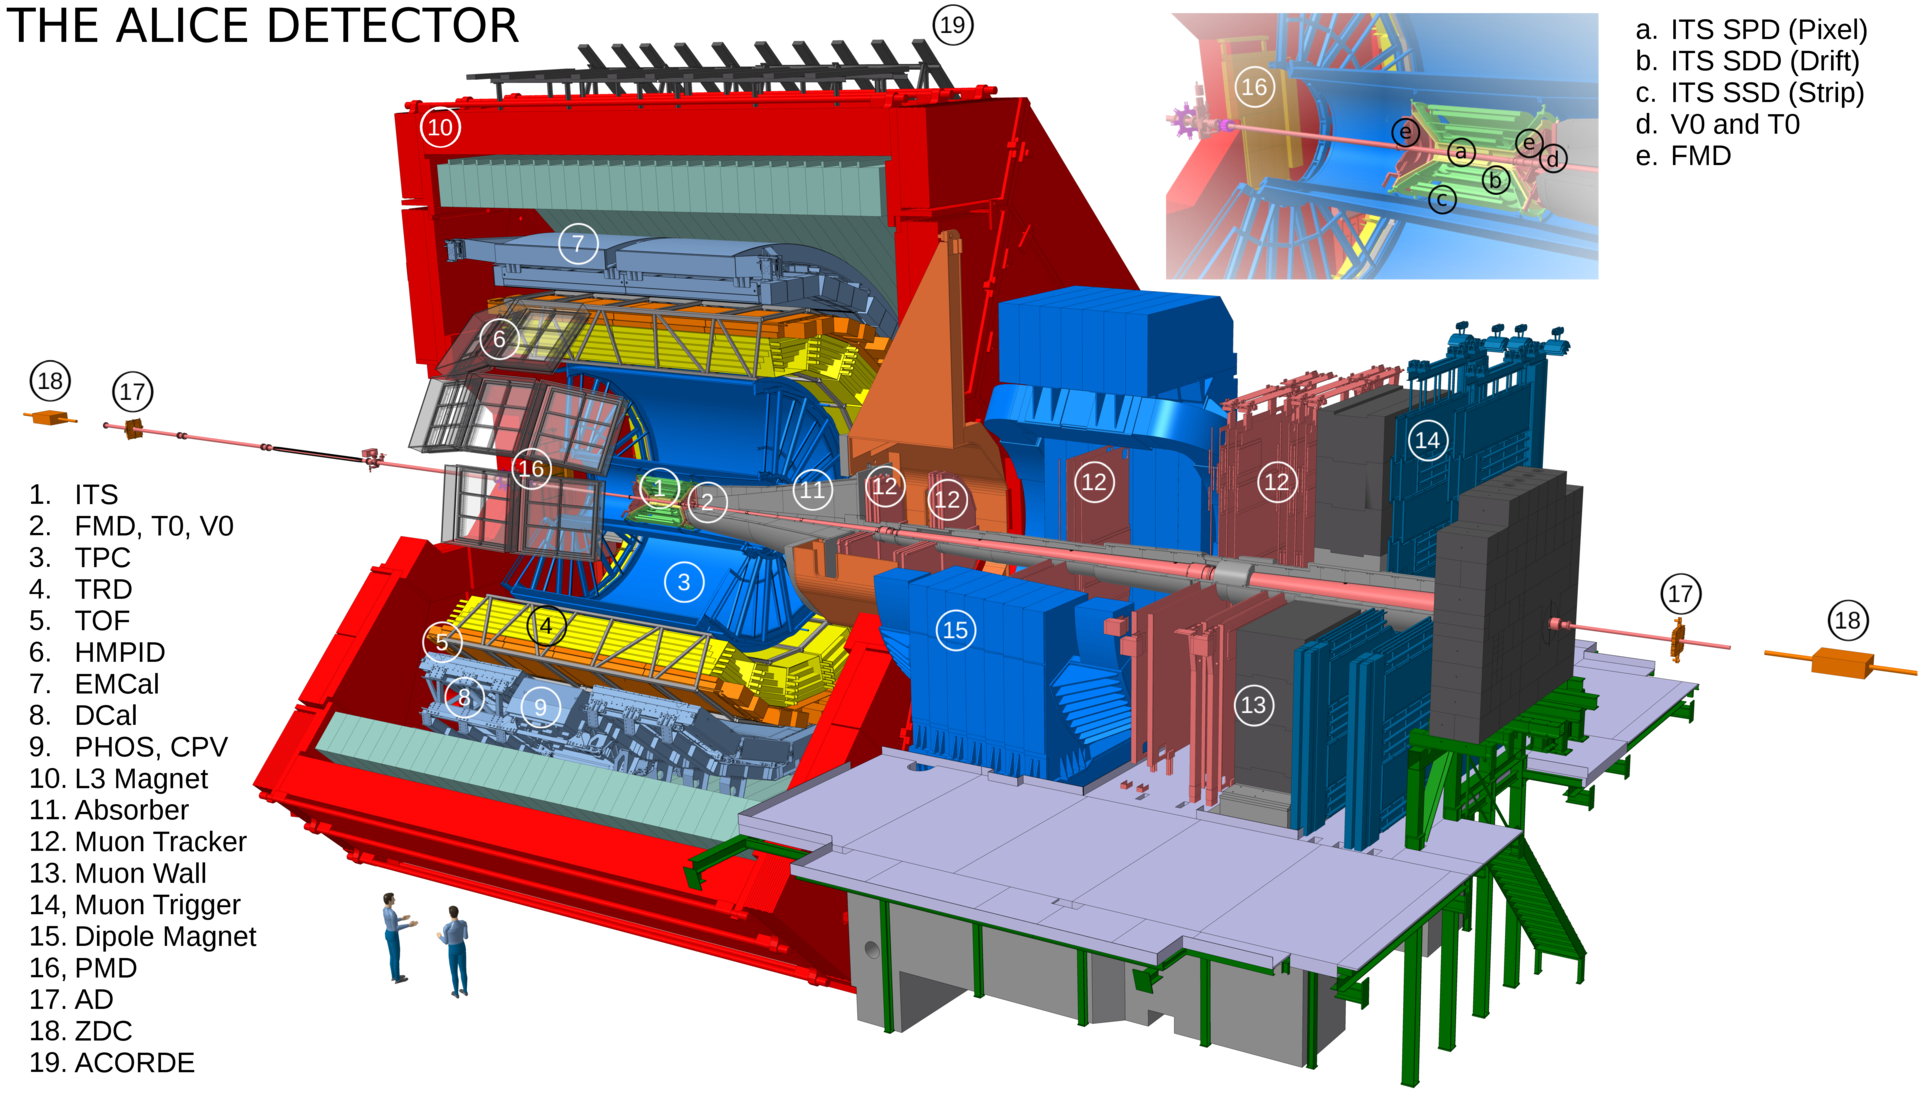
\includegraphics[width=.7\textwidth]{intro/2017-May-11-ALICE_RUN2_labels_HD}
\caption{Detector setup in Run 2}
\label{fig:alice_run2}
\end{figure}

\begin{figure}
\centering
\caption{tracking efficiency}
\label{fig:trk_eff}
\end{figure}

\begin{figure}
\centering
\caption{tracking \pt resolution}
\label{fig:trk_res}
\end{figure}

\subsection{Calorimetry}

\subsection{Particle identification}

\begin{figure}
\centering
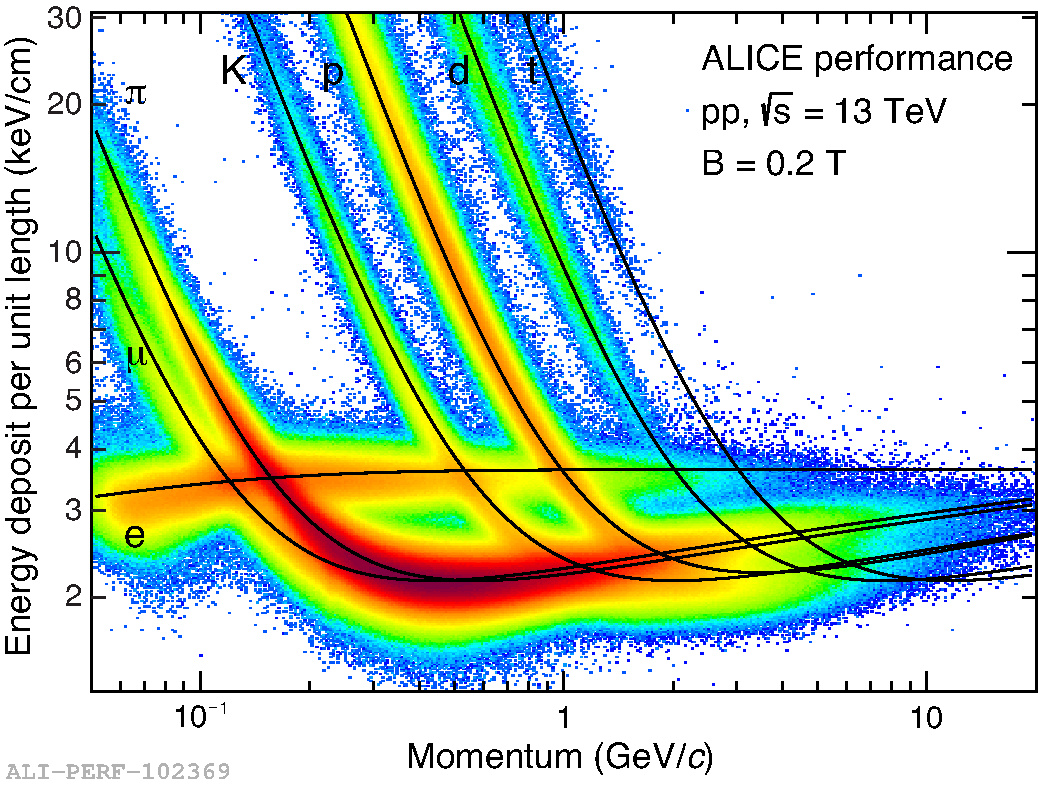
\includegraphics[width=.7\textwidth]{intro/2018-Jul-23-TPC_dEdx_2T_151003_color}
\caption{TPC dE/dx}
\label{fig:tpc_dedx}
\end{figure}

\subsection{Event characterization and selection}

\subsection{Forward spectrometer}

\subsection*{Run1/2 performance highlights (examples)}

cite performance paper~\cite{Abelev:2014ffa}, possibly also detector papers

discuss performance
\begin{itemize}
\item particle identification and relevant detectors
\item secondary vertex resolution
\item data sets (rate/integrated luminosity)
\end{itemize}

Data was recorded throughout the
running of the LHC in Run 1 and 2 exploiting a variety of collision systems and
energies, see Tab.~\ref{tab:datasets}.

\begin{figure}
\centering
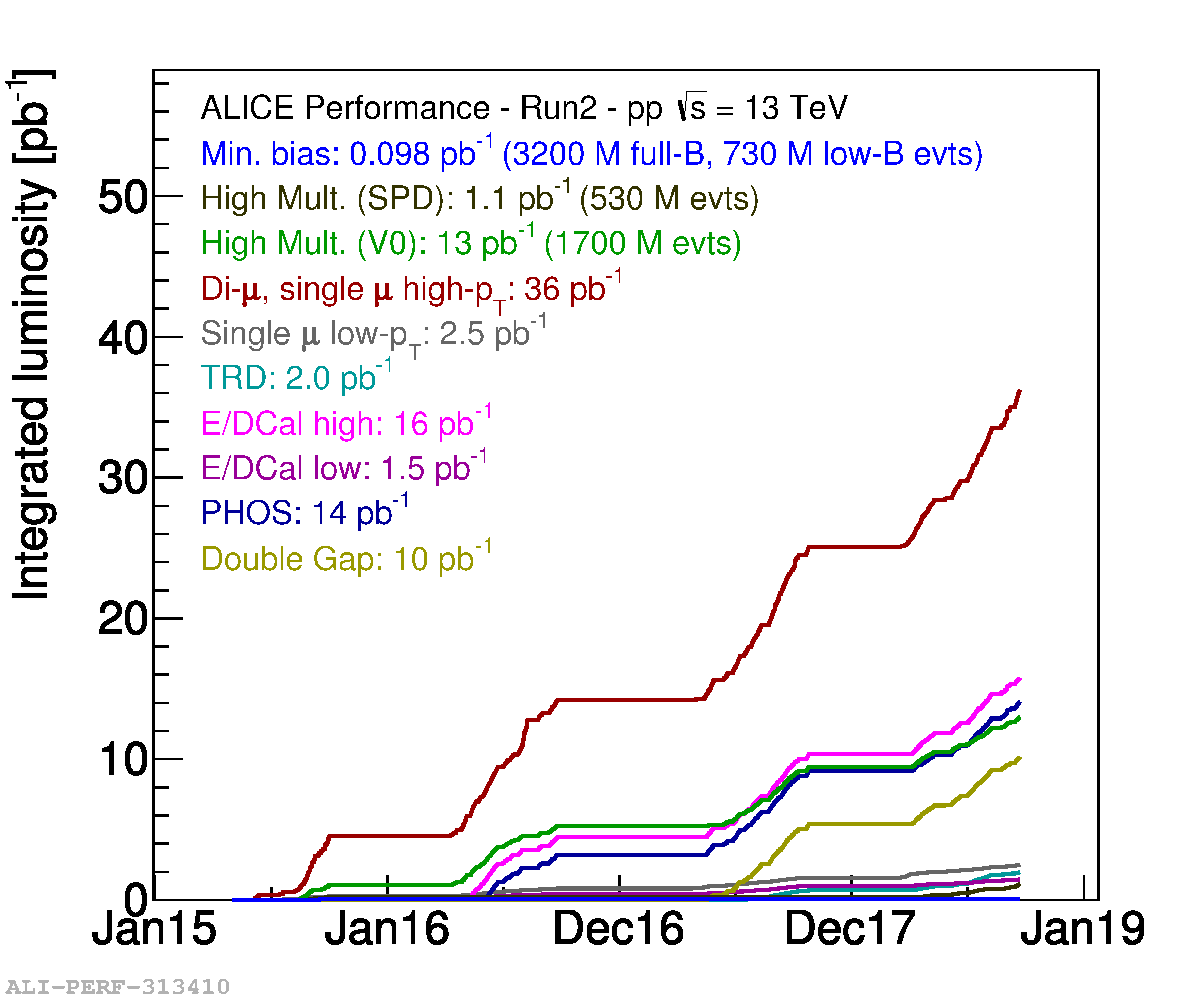
\includegraphics[width=.45\textwidth]{intro/2019-01-17-2019-01-17-lumi_Run2_pp13TeV}
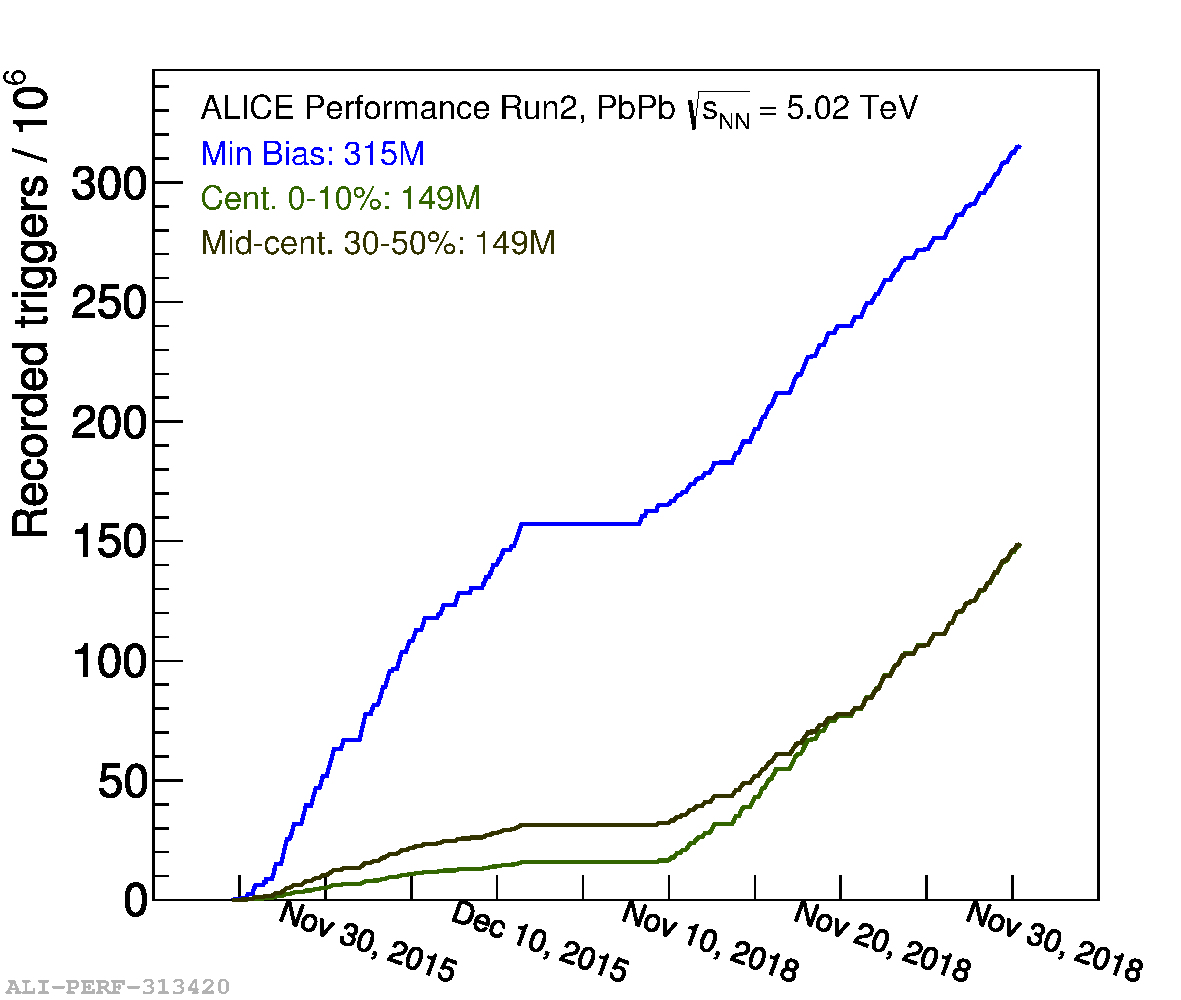
\includegraphics[width=.45\textwidth]{intro/2019-01-17-2019-01-17-stat_Run2_PbPb}
\caption{integrated lumi}
\label{fig:lumi_run2}
\end{figure}

\begin{table}
  \centering
  \begin{tabular}{lrrr}
    \multicolumn{1}{c}{system}
    & \multicolumn{1}{c}{$\snn~(\mathrm{\TeV})$}
    & \multicolumn{1}{c}{$L_\mathrm{MB}$}
    & \multicolumn{1}{c}{$L_\mathrm{insp}$}\\
    \hline \hline
    \pp & 0.9 & & $\sim 200~\mu\mathrm{b}^{-1}$\\
        & 2.76 & & $\sim 100~\mathrm{nb}^{-1}$\\
        & 5.02 & & $\sim 1.3~\mathrm{pb}^{-1}$\\
        & 7 & & $\sim 1.5~\mathrm{pb}^{-1}$\\
        & 8 & & $\sim 2.5~\mathrm{pb}^{-1}$\\
        & 13 & & $\sim 25~\mathrm{pb}^{-1}$\\
    \pPb{} & 5.02 & & $\sim 15 + 3~\mathrm{nb}^{-1}$\\
           & 8.16 & & $\sim 25~\mathrm{nb}^{-1}$\\
    \XeXe{} & 5.44 & & $\sim 0.3~\mu\mathrm{b}^{-1}$\\
    \PbPb{} & 2.76 & & $\sim 75~\mu\mathrm{b}^{-1}$\\
            & 5.02 & & $\sim 0.25 + 1~\mathrm{nb}^{-1}$\\
    \hline
  \end{tabular}
  \caption{ALICE datasets from LHC Run 1 and 2}
  \label{tab:datasets}
\end{table}
